\ifx\allfiles\undefined
\documentclass[12pt, a4paper, oneside, UTF8]{ctexbook}
\def\path{../../config}
\usepackage{amsmath}
\usepackage{amsthm}
\usepackage{amssymb}
\usepackage{array}
\usepackage{xcolor}
\usepackage{graphicx}
\usepackage{mathrsfs}
\usepackage{enumitem}
\usepackage{geometry}
\usepackage[colorlinks, linkcolor=black]{hyperref}
\usepackage{stackengine}
\usepackage{yhmath}
\usepackage{extarrows}
\usepackage{tikz}
\usepackage{pgfplots}
\usepackage{asymptote}
\usepackage{float}
\usepackage{fontspec} % 使用字体

\setmainfont{Times New Roman}
\setCJKmainfont{LXGWWenKai-Light}[
    SlantedFont=*
]

\everymath{\displaystyle}

\usepgfplotslibrary{polar}
\usepackage{subcaption}
\usetikzlibrary{decorations.pathreplacing, positioning}

\usepgfplotslibrary{fillbetween}
\pgfplotsset{compat=1.18}
% \usepackage{unicode-math}
\usepackage{esint}
\usepackage[most]{tcolorbox}

\usepackage{fancyhdr}
\usepackage[dvipsnames, svgnames]{xcolor}
\usepackage{listings}

\definecolor{mygreen}{rgb}{0,0.6,0}
\definecolor{mygray}{rgb}{0.5,0.5,0.5}
\definecolor{mymauve}{rgb}{0.58,0,0.82}
\definecolor{NavyBlue}{RGB}{0,0,128}
\definecolor{Rhodamine}{RGB}{255,0,255}
\definecolor{PineGreen}{RGB}{0,128,0}

\graphicspath{ {figures/},{../figures/}, {config/}, {../config/} }

\linespread{1.6}

\geometry{
    top=25.4mm, 
    bottom=25.4mm, 
    left=20mm, 
    right=20mm, 
    headheight=2.17cm, 
    headsep=4mm, 
    footskip=12mm
}

\setenumerate[1]{itemsep=5pt,partopsep=0pt,parsep=\parskip,topsep=5pt}
\setitemize[1]{itemsep=5pt,partopsep=0pt,parsep=\parskip,topsep=5pt}
\setdescription{itemsep=5pt,partopsep=0pt,parsep=\parskip,topsep=5pt}

\lstset{
    language=Mathematica,
    basicstyle=\tt,
    breaklines=true,
    keywordstyle=\bfseries\color{NavyBlue}, 
    emphstyle=\bfseries\color{Rhodamine},
    commentstyle=\itshape\color{black!50!white}, 
    stringstyle=\bfseries\color{PineGreen!90!black},
    columns=flexible,
    numbers=left,
    numberstyle=\footnotesize,
    frame=tb,
    breakatwhitespace=false,
} 

\lstset{
    language=TeX, % 设置语言为 TeX
    basicstyle=\ttfamily, % 使用等宽字体
    breaklines=true, % 自动换行
    keywordstyle=\bfseries\color{NavyBlue}, % 关键字样式
    emphstyle=\bfseries\color{Rhodamine}, % 强调样式
    commentstyle=\itshape\color{black!50!white}, % 注释样式
    stringstyle=\bfseries\color{PineGreen!90!black}, % 字符串样式
    columns=flexible, % 列的灵活性
    numbers=left, % 行号在左侧
    numberstyle=\footnotesize, % 行号字体大小
    frame=tb, % 顶部和底部边框
    breakatwhitespace=false % 不在空白处断行
}

% \begin{lstlisting}[language=TeX] ... \end{lstlisting}

% 定理环境设置
\usepackage[strict]{changepage} 
\usepackage{framed}

\definecolor{greenshade}{rgb}{0.90,1,0.92}
\definecolor{redshade}{rgb}{1.00,0.88,0.88}
\definecolor{brownshade}{rgb}{0.99,0.95,0.9}
\definecolor{lilacshade}{rgb}{0.95,0.93,0.98}
\definecolor{orangeshade}{rgb}{1.00,0.88,0.82}
\definecolor{lightblueshade}{rgb}{0.8,0.92,1}
\definecolor{purple}{rgb}{0.81,0.85,1}

\theoremstyle{definition}
\newtheorem{myDefn}{\indent Definition}[section]
\newtheorem{myLemma}{\indent Lemma}[section]
\newtheorem{myThm}[myLemma]{\indent Theorem}
\newtheorem{myCorollary}[myLemma]{\indent Corollary}
\newtheorem{myCriterion}[myLemma]{\indent Criterion}
\newtheorem*{myRemark}{\indent Remark}
\newtheorem{myProposition}{\indent Proposition}[section]

\newenvironment{formal}[2][]{%
	\def\FrameCommand{%
		\hspace{1pt}%
		{\color{#1}\vrule width 2pt}%
		{\color{#2}\vrule width 4pt}%
		\colorbox{#2}%
	}%
	\MakeFramed{\advance\hsize-\width\FrameRestore}%
	\noindent\hspace{-4.55pt}%
	\begin{adjustwidth}{}{7pt}\vspace{2pt}\vspace{2pt}}{%
		\vspace{2pt}\end{adjustwidth}\endMakeFramed%
}

\newenvironment{definition}{\vspace{-\baselineskip * 2 / 3}%
	\begin{formal}[Green]{greenshade}\vspace{-\baselineskip * 4 / 5}\begin{myDefn}}
	{\end{myDefn}\end{formal}\vspace{-\baselineskip * 2 / 3}}

\newenvironment{theorem}{\vspace{-\baselineskip * 2 / 3}%
	\begin{formal}[LightSkyBlue]{lightblueshade}\vspace{-\baselineskip * 4 / 5}\begin{myThm}}%
	{\end{myThm}\end{formal}\vspace{-\baselineskip * 2 / 3}}

\newenvironment{lemma}{\vspace{-\baselineskip * 2 / 3}%
	\begin{formal}[Plum]{lilacshade}\vspace{-\baselineskip * 4 / 5}\begin{myLemma}}%
	{\end{myLemma}\end{formal}\vspace{-\baselineskip * 2 / 3}}

\newenvironment{corollary}{\vspace{-\baselineskip * 2 / 3}%
	\begin{formal}[BurlyWood]{brownshade}\vspace{-\baselineskip * 4 / 5}\begin{myCorollary}}%
	{\end{myCorollary}\end{formal}\vspace{-\baselineskip * 2 / 3}}

\newenvironment{criterion}{\vspace{-\baselineskip * 2 / 3}%
	\begin{formal}[DarkOrange]{orangeshade}\vspace{-\baselineskip * 4 / 5}\begin{myCriterion}}%
	{\end{myCriterion}\end{formal}\vspace{-\baselineskip * 2 / 3}}
	

\newenvironment{remark}{\vspace{-\baselineskip * 2 / 3}%
	\begin{formal}[LightCoral]{redshade}\vspace{-\baselineskip * 4 / 5}\begin{myRemark}}%
	{\end{myRemark}\end{formal}\vspace{-\baselineskip * 2 / 3}}

\newenvironment{proposition}{\vspace{-\baselineskip * 2 / 3}%
	\begin{formal}[RoyalPurple]{purple}\vspace{-\baselineskip * 4 / 5}\begin{myProposition}}%
	{\end{myProposition}\end{formal}\vspace{-\baselineskip * 2 / 3}}


\newtheorem{example}{\indent \color{SeaGreen}{Example}}[section]
\renewcommand{\proofname}{\indent\textbf{\textcolor{TealBlue}{Proof}}}
\NewEnviron{solution}{%
	\begin{proof}[\indent\textbf{\textcolor{TealBlue}{Solution}}]%
		\color{blue}% 设置内容为蓝色
		\BODY% 插入环境内容
		\color{black}% 恢复默认颜色(可选,避免影响后续文字)
	\end{proof}%
}

% 自定义命令的文件

\def\d{\mathrm{d}}
\def\R{\mathbb{R}}
%\newcommand{\bs}[1]{\boldsymbol{#1}}
%\newcommand{\ora}[1]{\overrightarrow{#1}}
\newcommand{\myspace}[1]{\par\vspace{#1\baselineskip}}
\newcommand{\xrowht}[2][0]{\addstackgap[.5\dimexpr#2\relax]{\vphantom{#1}}}
\newenvironment{mycases}[1][1]{\linespread{#1} \selectfont \begin{cases}}{\end{cases}}
\newenvironment{myvmatrix}[1][1]{\linespread{#1} \selectfont \begin{vmatrix}}{\end{vmatrix}}
\newcommand{\tabincell}[2]{\begin{tabular}{@{}#1@{}}#2\end{tabular}}
\newcommand{\pll}{\kern 0.56em/\kern -0.8em /\kern 0.56em}
\newcommand{\dive}[1][F]{\mathrm{div}\;\boldsymbol{#1}}
\newcommand{\rotn}[1][A]{\mathrm{rot}\;\boldsymbol{#1}}

\newif\ifshowanswers
\showanswerstrue % 注释掉这行就不显示答案

% 定义答案环境
\newcommand{\answer}[1]{%
    \ifshowanswers
        #1%
    \fi
}

% 修改参数改变封面样式,0 默认原始封面、内置其他1、2、3种封面样式
\def\myIndex{0}


\ifnum\myIndex>0
    \input{\path/cover_package_\myIndex} 
\fi

\def\myTitle{考研数学笔记}
\def\myAuthor{Weary Bird}
\def\myDateCover{\today}
\def\myDateForeword{\today}
\def\myForeword{相见欢·林花谢了春红}
\def\myForewordText{
    林花谢了春红,太匆匆。
    无奈朝来寒雨晚来风。
    胭脂泪,相留醉,几时重。
    自是人生长恨水长东。
}
\def\mySubheading{以姜晓千强化课讲义为底本}


\begin{document}
\input{\path/cover_text_\myIndex.tex}

\newpage
\thispagestyle{empty}
\begin{center}
    \Huge\textbf{\myForeword}
\end{center}
\myForewordText
\begin{flushright}
    \begin{tabular}{c}
        \myDateForeword
    \end{tabular}
\end{flushright}

\newpage
\pagestyle{plain}
\setcounter{page}{1}
\pagenumbering{Roman}
\tableofcontents

\newpage
\pagenumbering{arabic}
% \setcounter{chapter}{-1}
\setcounter{page}{1}

\pagestyle{fancy}
\fancyfoot[C]{\thepage}
\renewcommand{\headrulewidth}{0.4pt}
\renewcommand{\footrulewidth}{0pt}








\else
\fi

\chapter{常微分方程}
\section{一阶微分方程}
\begin{remark}
    一阶微分方程 \\
    (一)可分离变量类型: 形如$\displaystyle\frac{\d y}{\d x}=f(x)g(y)$ 可以转换为 $\displaystyle \frac{\d y}{g(y)}=f(x)\d x$ \\
    (二)一阶线性非齐次: 形如$y'+p(x)y=q(x)$ 其通解公式为
    $$
    \color{red}
    y=e^{-\int p(x)\d x}\left[\int e^{\int p(x)\d x}q(x)\d x + C\right]
    $$
    特殊的,一阶线性齐次$y'+p(x)y=0$其通解公式为
    $$
    \color{red}
    y=Ce^{-\int p(x)\d x}
    $$
    (三)一阶齐次方程: 形如$\displaystyle y' = f(\frac{y}{x})$ 则可以通过${\displaystyle\color{red}u=\frac{y}{x}}$为可分离变量类型 \\
    (四)全微分方程: 形如$P(x,y)\d x + Q(x,y)\d y = 0,$且$\displaystyle \frac{\d Q}{\d x}=\frac{\d P}{\d y}$ 则其解法本质都是求原函数 
    \begin{enumerate}
        \item [(I)] 特殊路径积分法 $\displaystyle u(x,y)=\int_{x_0}^{x}P(x,y_0)\d x + \int_{y_0}^{y}Q(x,y)\d y$ 
        \item [(II)] {\color{red} 偏积分, 一般考虑直接偏积分}
        \item [(III)] 凑微分
    \end{enumerate}
    (五)伯努利方程: 形如$y'(x)+p(x)y=q(x)y^{\alpha},\alpha\neq (0, 1)$ 其解法如下 
    \begin{enumerate}
        \item [(I)] 同除$y^{\alpha}$,转换为$y^{-\alpha}y'+p(x)y^{1-\alpha}=q(x)$
        \item [(II)] 做$\color{red}z=y^{1-\alpha}$的换元,则原微分方程转换为 
        \item [(III)] $\displaystyle \frac{\d z}{\d x} + (1-\alpha)p(x)z=(1-\alpha)q(x)$ 
        \item [(IV)] 转换为一阶线性方程可以用公式法直接求
    \end{enumerate}
    (六)需要考虑变量互换: 形如
    $$
    \frac{\d y}{\d x} = \frac{h(y)}{p(y)x + q(y)}, \frac{\d y}{\d x}=\frac{h(y)}{p(y)x+q(y)x^{\alpha}}
    $$
    交换后可以转换为一阶线性/一阶伯努利 即
    $$
    \frac{\d x}{\d y} = \frac{p(y)}{h(y)} + \frac{q(y)}{h(y)}, \frac{\d x}{\d y} = \frac{p(y)}{h(y)} + \frac{q(y)}{h(y)}x^{\alpha}
    $$
\end{remark}
\begin{enumerate}[label=\arabic*.]
    \item (1998,数一、数二)已知函数$y=y(x)$在任意点$x$处的增量$\Delta y=\frac{y\Delta x}{1+x^2}+\alpha$,其中$\alpha$是$\Delta x$的高阶无穷小,$y(0)=\pi$,则$y(1)$等于 \\
    $(A)\ 2\pi \quad (B)\ \pi \quad (C)\ e^{\frac{\pi}{4}} \quad (D)\ \pi e^{\frac{\pi}{4}}$

    \begin{solution}
    两边同除$\Delta x$且当$\Delta x\to 0$,有$\displaystyle y'=\frac{y}{1+x^2}$ 原问题转换为求初值问题的解
    $$
    \begin{cases}
        \displaystyle y' - \frac{y}{1+x^2} = 0 \\
        y(0)=\pi
    \end{cases}
    $$
    由公式有$\displaystyle y=\pi e^{\frac{\pi}{4}}$ 
    \end{solution}
    
    \item (2002,数二)已知函数$f(x)$在$(0,+\infty)$内可导,$f(x)>0$,$\displaystyle\lim_{x\to+\infty}f(x)=1$,且满足
    \begin{align*}
        \lim_{h\to0}\left(\frac{f(x+hx)}{f(x)}\right)^{\frac{1}{h}}=e^{\frac{1}{x}}
    \end{align*}
    求$f(x)$。
    
    \begin{solution}
    由题设有
    \begin{align*}
        \text{原式} &= e^{\displaystyle\lim_{h\to 0}\frac{f(x+hx)-f(x)}{hf(x)}} \\
        &=e^{\frac{f'(x)\cdot x}{x}} = e^{\frac{1}{x}} \implies \frac{f'(x)\cdot x}{f(x)}=\frac{1}{x}
    \end{align*}
    即原问题转换为如下初值问题的解
    $$
    \begin{cases}
        \displaystyle 
        f'(x) - \frac{1}{x^2}\cdot f(x) = 0 \\
        \displaystyle
        \lim_{x\to\infty}f(x) = 1
    \end{cases}
    $$
    带入公式有$\displaystyle f(x)=e^{-\frac{1}{x}}$
    \end{solution}
\end{enumerate}

\begin{enumerate}[label=\arabic*.,start=3]
    \item (1999,数二)求初值问题
    \begin{align*}
        \begin{cases}
            (y+\sqrt{x^2+y^2})dx-xdy=0 & (x>0) \\
            y|_{x=1}=0
        \end{cases}
    \end{align*}
    
    \begin{solution}
    等式两边同时除以x,原式化为
    $$
    \left[\frac{y}{x}+\sqrt{1+(\frac{y}{x})^2}\right]\d x = \d y 
    $$
    令$u=\frac{y}{x}$,则$\frac{\d y}{\d x} = u + x\frac{\d u}{\d x}$ 原式化为
    $$
    \frac{\d u}{\sqrt{1+u^2}} = \frac{\d x}{x}
    $$
    两边同时积分
    $$
    \begin{cases}
        \displaystyle\frac{y}{x}+\sqrt{1+(\frac{y}{x})^2}=Cx \\
        \displaystyle y(1) = 0
    \end{cases} \implies y + \sqrt{x^2+y^2}=x^2
    $$
    {\color{red} 对于带有根式的结果特别需要注意化简,两边同时乘以 $y - \sqrt{x^2+y^2}$,可以解出$y=\frac{1}{2}(x^2+1)$}
    \end{solution}
\end{enumerate}



\begin{enumerate}[label=\arabic*.,start=4]
    \item (2010,数二、数三)设$y_1,y_2$是一阶线性非齐次微分方程$y'+p(x)y=q(x)$的两个特解。若常数$\lambda,\mu$使$\lambda y_1+\mu y_2$是该方程的解,$\lambda y_1-\mu y_2$是该方程对应的齐次方程的解,则 \\
    $(A)\ \lambda=\frac{1}{2},\ \mu=\frac{1}{2} \qquad (B)\ \lambda=-\frac{1}{2},\mu=-\frac{1}{2}$ \\
    $(C)\ \lambda=\frac{2}{3},\ \mu=\frac{1}{3}\qquad (D)\ \lambda=\frac{2}{3},\mu=\frac{2}{3}$ 

    
    \begin{solution}
    由总结可知,选A
    \end{solution}

    \begin{tcolorbox}[title={一阶,二阶线性微分方程(组)解的性质}]
    若$y_1,y_2$分别为非齐次特解,则
    $$
    C_1y_1+C_2y_2 \begin{cases}
        C_1 + C_1 = 0, & \text{齐次解} \\
        C_1 + C_2 = 1, & \text{非齐次解}
    \end{cases}
    $$
    \end{tcolorbox}
\end{enumerate}

\begin{enumerate}[label=\arabic*.,start=5]
    \item (2018,数一)已知微分方程$y'+y=f(x)$,其中$f(x)$是$\mathbb{R}$上的连续函数。
    \begin{enumerate}[label=(\roman*)]
        \item[(1)] 若$f(x)=x$,求方程的通解;
        \item[(2)] 若$f(x)$是周期为$T$的函数,证明:方程存在唯一的以$T$为周期的解。
    \end{enumerate}
    
    \begin{solution}
    (一)由一阶线性的求解公式有 
    \begin{align*}
        y &= e^{-x}\left[\int e^x\cdot x\d x + C\right] \\
        &=e^{-x}\left[(x-1)e^{-x}+C\right]\\
        &=Ce^{-x}+x-1
    \end{align*}
    (二)由一阶线性的求解公式有
    $$
    y=e^{-x}\left[\int f(x)e^{x}\d x + C\right] = {\color{red} e^{-x}\int_{0}^{x}e^{t}f(t)\d t+C}
    $$
    则
    \begin{align*}
        y(x+T)-y(x) &= e^{-x}\left[\frac{1}{e^T}\int_{0}^{x+T}e^{t}f(t)\d t - 
        \int_{0}^{x}e^{t}f(t)\d t + (\frac{1}{e^{T}-1})C\right] \\
        \int_{0}^{x+T}e^{t}f(t)\d t &=\int_{0}^{T}+\int_{T}^{x+T} \\
        &=\frac{1}{e^{t}}\int_{0}^{T}e^{t}f(t)\d t + \frac{1}{e^T}\int_{T}^{x+T}e^{T}f(t)\d t \\
        &=\ldots + \frac{1}{e^T}\int_{0}^{T}e^{t+T}f(t+T)\d t \\
        y(x+T)-y(x) & = e^{-x}\left[\frac{1}{e^{T}}\int_{0}^{T}e^{t}f(t)\d t + (\frac{1}{e^{T}-1})C \right] 
    \end{align*}
    由周期函数的定义,只需要令$y(x+T)-y(x)=0$即
    $$
    C = -\frac{1}{1-e^T}\int_{0}^{T}e^tf(t)\d t
    $$
    的时候该方程的解是周期还是,且唯一.
    \end{solution}
\end{enumerate}


\begin{enumerate}[label=\arabic*.,start=6]
    \item 求解微分方程$y'-\frac{4}{x}y=x^2\sqrt{y}$.
    
    \begin{solution}
    令$z=\sqrt{y}$,则$\displaystyle z'-\frac{2}{x}z=\frac{1}{2}x^2$,则到
    $$\displaystyle
    z = e^{\int\frac{2}{x}\d x}\left(\int\frac{1}{2}x^2e^{-\int\frac{2}{x}\d x}\d x + C\right) 
    =x^2\left(\frac{1}{2}\cdot x + C\right)
    $$
    则该方程的通解为$\sqrt{y}=\frac{1}{2}x^3+Cx^2$
    \end{solution}
\end{enumerate}

\begin{enumerate}[label=\arabic*.,start=7]
    \item 求解下列微分方程:\\
        $(1)\ (2xe^y+3x^2-1)dx+(x^2e^y-2y)dy=0;$ \\
        $(2)\ \frac{2x}{y^3}dx+\frac{y^2-3x^2}{y^4}dy=0$.
    
    \begin{solution}
    (1) 偏积分法 
    $$
    u(x,y)=\int(2xe^y+3x^2-1)\d x = x^2e^y+x^3-x+\phi(y)
    $$
    由于$\displaystyle \frac{\partial u}{\partial y} = x^2e^y + \phi'(y)$对比题目可知
    $\phi'(y)=-2y\implies\phi(y)=-y^2$,故原方程的解
    $$
    x^2e^y+x^3-x-y^2=C
    $$
    (2) 凑微分法
    \begin{align*}
    \text{原式} 
    &=(2xe^y+3x^2-1)\d x + (x^2e^y-2y)\d y  \\
    &= (2xe^y\d x + x^2e^y\d y)+(3x^2-1)\d x + (-2y)\d y \\
    &=d(x^2e^y)+d(x^3-x)+d(-y^2) \\
    &=d(x^2e^y+x^3-x-y^2) = 0
    \end{align*}
    即$x^2e^y+x^3-x-y^2=C$
    \end{solution}
\end{enumerate}

\section{二阶常系数线性微分方程}
\begin{remark}
    二阶齐次方程的通解,形如$y''+py'+qy=0$ \\
    求解特征方程($r^2+pr+q=0$)
    $$
    \begin{cases}
        r_1\neq r_2, & \text{通解为} C_1e^{r_1 x} + C_2e^{r_2 x} \\
        r_1=r_2=r, & \text{通解为} (C_1 + C_2 x)e^{rx} \\
        r_{1,2}=\alpha\pm\beta, &\text{通解为} e^{\alpha x}(C_1\cos{\beta x}+C_2\sin{\beta x})
    \end{cases}
    $$
    二阶非齐次方程的通解,形如$y''+py'+qy=f(x)$,其解的结构为\underline{齐次特解 + 非齐次通解}
    $$
    \text{特解格式}
    \begin{cases}
        f(x)=P_ne^{\lambda x},y^{*}=x^kQ_n(x)e^{\lambda x} \\
        f(x)=e^{\alpha x}[P_{m}(x)\cos{\beta x}+P_{n}(x)\sin{\beta x}] \\
        y^{*}=x^ke^{\alpha}[Q_{l}(x)\cos{\beta x}+R_{l}(x)\sin{\beta x}], l = \min{\{m,n\}}
    \end{cases}
    $$
\end{remark}
\begin{enumerate}[label=\arabic*.,start=8]
    \item (2017,数二)微分方程$y''-4y'+8y=e^{2x}(1+\cos2x)$的特解可设为$y^*=$ \\
        $(A)\ Ae^{2x}+e^{2x}(B\cos2x+C\sin2x)$ \\
        $(B)\ Axe^{2x}+e^{2x}(B\cos2x+C\sin2x)$ \\
        $(C)\ Ae^{2x}+xe^{2x}(B\cos2x+C\sin2x)$ \\
        $(D)\ Axe^{2x}+xe^{2x}(B\cos2x+C\sin2x)$
    
    \begin{solution}
    原方程可以转换为如下两式的和
    \begin{align}
        y'' - 4y' + 8y &= e^2x \\
        y'' - 4y' + 8y &= e^2x\cdot\cos{2x}
    \end{align}
    解特征方程有
    $$
    r^2-4r+8=0 \implies r_{1,2}=\frac{4+\sqrt{-16}}{2}=2\pm 2i
    $$
    则上述两个方程的特解分别为
    \begin{align*}
        y_1^{*} &=Ae^{2x} \\
        y_2^{*} &=xe^{2x}(B\sin{2x}+C\cos{2x}) 
    \end{align*}
    由\underline{叠加原理}可知,原方程的特解为
    $$
    y^{*}=Ae^{2x}+xe^{2x}(B\sin{2x}+C\cos{2x}) 
    $$
    \end{solution}
    
    \item (2015,数一)设$y=\frac{1}{2}e^{2x}+(x-\frac{1}{3})e^x$是二阶常系数非齐次线性微分方程$y''+ay'+by=ce^x$的一个特解,则 \\
    $(A)\ a=-3,b=2,c=-1$ \qquad
    $(B)\ a=3,b=2,c=-1$ \\
    $(C)\ a=-3,b=2,c=1$ \qquad
    $(D)\ a=3,b=2,c=1$ 
    
    \begin{solution}
    (方法一) 带入原方程求解a,b,c即 
    $$
    \begin{cases}
        y=\frac{1}{2}e^{2x}+(x-\frac{1}{3})e^x \\
        y'=e^{2x}+(x+\frac{2}{3})e^x \\
        y''=2e^{2x}+(x+\frac{5}{3})e^x \\
        y''+ay'+by=ce^x 
    \end{cases} \implies \begin{cases}
        2+a+\frac{b}{2} = 0 \\
        1+a+b = 0 \\
        \frac{5}{3}+\frac{2a}{3}-\frac{b}{3} = c 
    \end{cases} \implies \begin{cases}
        a = -3 \\
        b = 2 \\
        c = -1
    \end{cases}
    $$
    (方法二)利用解的特性反推微分方程 
    $$
    y=\frac{1}{2}e^{2x}-\frac{1}{3}e^x+xe^x
    $$
    显然其齐次方程的解为$\displaystyle \frac{1}{2}e^{2x}-\frac{1}{3}e^x$,非齐次特解为 $xe^x$,故可以推导出该
    微分方程的齐次通解为$C_1e^{2x}+C_2e^x$,则其特征方程为$(r-2)(r-1)=0$,从而可知$a=-3,b=2$,将非齐次特解带入可以求出$c=-1$
    \end{solution}
    
    \item (2016,数二)已知$y_1(x)=e^x$,$y_2(x)=u(x)e^x$是二阶微分方程$(2x-1)y''-(2x+1)y'+2y=0$的两个解。若$u(-1)=e$,$u(0)=-1$,求$u(x)$,并写出该微分方程的通解。
    
    \begin{solution}
    将$y_2(x)$以及如下带入原方程有
    $$
    \begin{cases}
        y'_2(x) = e^x\left[u'(x)+u(x)\right] \\
        y''_2(x) = e^x\left[u''(x)+2u'(x)+u(x)\right]
    \end{cases}
    $$
    有
    $$
    (2x-1)u''(x)+(2x-3)u'(x) = 0
    $$
    (方法一)典型的可降阶方程,令$u'(x)=p$ 有
    $$
    (2x-1)p'+(2x-3)p = 0 \implies p = Ce^{-\int\frac{2x-3}{2x-1}\d x} = u'(x)
    $$

    (方法二)分离变量
    $$
    \int\frac{u''(x)}{u'(x)}\d x = \int -\frac{2x-3}{2x-1}\d x 
    $$
    即$\ln{\left|u'(x)\right|} = \ln{\left|2x-1\right|} - x + \ln{\left|C_1\right|}$

    $$
    u(x)=\int u'(x)\d x = -C_1(1+2x)e^{-x} + C_2 
    $$
    带入初值条件有
    $$
    \fbox{$u(x)=-(2x+1)e^{-x}$}
    $$
    \end{solution}
    
    \item (2016,数一)设函数$y(x)$满足方程$y''+2y'+ky=0$,其中$0<k<1$。
    \begin{enumerate}[label=(\roman*)]
        \item[(1)] 证明反常积分$\int_0^{+\infty}y(x)dx$收敛;
        \item[(2)] 若$y(0)=1$,$y'(0)=1$,求$\int_0^{+\infty}y(x)dx$的值。
    \end{enumerate}
    
    \begin{solution}
    (1)解特征方程$r^2+2r+k=0$又$0<k<1$故特征方程的解为
    $$
        r_{1,2}=-1\pm\sqrt{1-k}
    $$
    从而该方程的齐次通解为
    $$
        y=C_1e^{r_1x}+C_2^{r_2x}
    $$
    方法一:直接计算方常积分
    \begin{align*}
        \int_{0}^{\infty}\left(C_1e^{r_1x}+C_2e^{r_2x}\right)\d x 
        &= \left(\frac{C_1}{r_1}e^{r_1 x}+\frac{C_2}{r_2}e^{r_2 x}\right)\bigg|^{+\infty}_{0} \\
        &\xlongequal{r_{1,2}<0} -\left(\frac{C_1}{r_1}+\frac{C_2}{r_2}\right) 
    \end{align*}
    故原反常积分收敛  \\
    方法二:用比较判别法
    $$
    \lim_{x\to\infty}x^p(C_1e^{r_1x}+C_2e^{r_2x})
    $$
    又$r_{1,2}<0$上式恒为0,又$p=2$的时候$\displaystyle\int_{1}^{+\infty}\frac{1}{x^2}\d x$收敛由比较判别法可知
    原反常积分收敛 \\
    (2)
    方法一: 尝试求根并计算 由$y(0)=y'(0)=1$有
    $$
    \begin{cases}
        C_1+C_2=1 \\
        r_1C_1+r_2C_2 = 1
    \end{cases} \implies \begin{cases}
        C_1=\frac{r_2-1}{r_2-r_1} \\
        C_2=\frac{1-r_1}{r_2-r_1}
    \end{cases}
    $$
    此时$C_1r_1+C_2r_2=r_1+r_2-1$带入积分有
    $$
    \int_{0}^{+\infty}y(x)\d x = -\frac{C_1r_2+C_2r_1}{r_1r_2}=-\frac{r_1+r_2-1}{r_1r_2}
    $$
    则由韦达定理有
    $\begin{cases}
    r_1+r_2 = -2 \\
    r_1r_2=k
    \end{cases}
    $
    则原反常积分为$\displaystyle\frac{3}{k}$

    方法二: 利用微分方程替换,
    带入$\displaystyle y=\frac{-1}{k}(y''+2y')$此时反常积分转换为
    \begin{align*}
        \int_{0}^{+\infty}-\frac{1}{k}(y''+2y')\d x 
        &= -\frac{1}{k}(y'+2y)\bigg|^{+\infty}_{0} \\
        &= \frac{3}{k}
    \end{align*}
    \end{solution}
\end{enumerate}

\section{ 高阶常系数线性齐次微分方程}

\begin{enumerate}[label=\arabic*.,start=12]
    \item 求解微分方程$y^{(4)}-3y''-4y=0$。
    
    \begin{solution}
    高阶齐次的解法和二阶齐次的解法完全一致,解特征方程判断解的结构 \\
    该微分方程的特征方程为
    $$
    r^4-3r^2-4=0 \implies (r-2)(r+2)(r^2+1)=0 \implies \begin{cases}
        r_1 = 2 \\
        r_2 = -2 \\
        r_{3,4} = \pm i 
    \end{cases}
    $$
    故原方程的通解为 
    $$
    y = C_1e^{2x}+C_2e^{-2x}+C_3\cos{x}+C_4\sin{x}
    $$
    \end{solution}
\end{enumerate}

\section{ 二阶可降阶微分方程}
\begin{remark}
    有两种类型 \\
    (一)缺$y$型 $y''=f(x,y')$ 令$y'=p$,则$p'=f(x,p)$ \\
    (二)缺$x$型 $y''=f(y',y)$ 令$y'=p$ 则$\displaystyle y''=p\frac{\d p}{\d y}$
\end{remark}
\begin{enumerate}[label=\arabic*.,start=13]
    \item 求微分方程$y''(x+y'^2)=y'$满足初始条件$y(1)=y'(1)=1$的特解。
    
    \begin{solution}
    本题不含$y$,令$y'=p,y''=p'$则原方程化简为$p'(x+p^2)=p$转换为反函数即
    $$
    \frac{\d x}{\d p}-\frac{1}{p}\cdot x=p \implies x = p(p+C)
    $$
    又$p(1)=p'(1)=1$可知$C=0$,从而$x=p^2\implies y'=\sqrt{x}$,从而$\displaystyle y=\frac{2}{3}x^{\frac{3}{2}}+C_1$又$y(1)=1$
    可知$\displaystyle y=\frac{2}{3}x^{\frac{3}{2}}+\frac{1}{3}$ 则 
    \end{solution}
\end{enumerate}

\newpage
\section{ 欧拉方程}
\begin{remark}
    对于形如
    $$
    x^ny^{(n)}+P_1x^{n-2}y^{(n-1)}\ldots+P_{n-1}xy'+P_ny=f(x)
    $$
    {\color{red} 令$x=e^t$},记$\displaystyle D=\frac{\d}{\d t}$
    $$
    \begin{cases}
        xy' = Dy \\
        x^2y'' = D(D-1)y \\
        \ldots \\
        x^ny^{(n)} = D(D-1)(D-2)\ldots(D-n+1)y
    \end{cases}
    $$
    一般只需要将$D\rightarrow r$求解特征方程即可,注意换元.
\end{remark}
\begin{enumerate}[label=\arabic*.,start=14]
    \item 求解微分方程$x^2y''+xy'+y=2\sin\ln x$。
    
    \begin{solution}
    {\color{red} 令$x=e^t$},则原方程转换为$D(D-1)y+Dy+y=2\sin{t}$ 特征方程为
    $$
    r(r-1)+r+1=0 \implies r_{1,2}=\pm i
    $$
    齐次方程的通解为$y=C_1\cos{t}+C_2\sin{t}$,令$y^{*}=t(A\cos{t}+B\sin{t})$,带入方程有$A=-1,B=0$故原方程的通解为
    $y=C_1\cos{\ln{x}}+C_2\sin{\ln{x}}-\ln{x}\cdot\cos{\ln{x}}$
    \end{solution}
\end{enumerate}

\section{ 变量代换求解二阶变系数线性微分方程}

\begin{enumerate}[label=\arabic*.,start=17]
    \item (2005,数二)用变量代换$x=\cos t(0<t<\pi)$化简微分方程$(1-x^2)y''-xy'+y=0$,并求其满足$y|_{x=0}=1$,$y'|_{x=0}=2$的特解。
    
    \begin{solution}
    有题设可知
    $$
    \begin{cases}
        \frac{\d y}{\d x}=\frac{\d y}{\d t}\frac{\d t}{\d x}=-\frac{1}{\sin{t}}\frac{\d y}{\d t} \\
        \frac{\d^2 y}{\d x^2} = -\frac{1}{\sin{t}}\left(\frac{\cos{t}}{\sin^2{t}}\frac{\d y}{\d t}-\frac{1}{\sin{t}}\frac{\d^2 y}{\d t^2}\right)
    \end{cases}
    $$
    代入方程有
    $$
    y''(t)+y(t) = 0 \implies y = C_1\cos{t}+C_2\sin{t} = C_1x+C_2\sqrt{1-x^2}
    $$
    带入题设初值条件,可知$y=2x+\sqrt{1-x^2}$
    \end{solution}
\end{enumerate}

\section{ 微分方程综合题}
\begin{enumerate}[label=\arabic*.,start=18]
    \item (2001,数二)设$L$是一条平面曲线,其上任意一点$P(x,y)(x>0)$到坐标原点的距离,恒等于该点处的切线在$y$轴上的截距,且$L$经过点$(\frac{1}{2},0)$。求曲线$L$的方程。
    
    \begin{solution}
    由题可设切线方程为
    $$
    Y-y=y'(X-x)
    $$
    令$x=0$,则$Y=-xy'+y$ 由题设原问题转换为如下初值问题的解
    $$
        \begin{cases}
        y-xy'=\sqrt{x^2+y^2} \\
        y(\frac{1}{2})=0
        \end{cases}
    $$
    可以解出$\displaystyle y=-x^2+\frac{1}{4}$
    \end{solution}
\end{enumerate}

\begin{enumerate}[label=\arabic*.,start=19]
    \item (2009,数三)设曲线$y=f(x)$,其中$f(x)$是可导函数,且$f(x)>0$。已知曲线$y=f(x)$与直线$y=0$,$x=1$及$x=t(t>1)$所围成的曲边梯形绕$x$轴旋转一周所得的立体体积值是该曲边梯形面积值的$\pi t$倍,求该曲线的方程。
    
    \begin{solution}
    有题设可以得到
    $$
    \pi\int_{1}^{t}f^{2}(x)\d x = \pi t\int_{1}^{t}f(x)\d x
    $$
    两边同时求导有
    $$
    f^{2}(t)=\int_{1}^{t}f(x)\d x+tf(t)
    $$
    {\color{red} 变限积分要注意其可能隐藏初值条件} 由$f(x)>0$可知$f(1)=1$ 再求导,此时原问题转换为如下初值问题的解
    $$
        \begin{cases}
            2f(t)f'(t)=tf'(t)+2f(t) \\
            f(1) = 1
        \end{cases}
    $$
    可以解出$\displaystyle x=\frac{2}{3}y+\frac{1}{3\sqrt{y}}$
    \end{solution}
\end{enumerate}

\begin{enumerate}[label=\arabic*.,start=20]
    \item (2016,数三)设函数$f(x)$连续,且满足$\int_0^x f(x-t)dt=\int_0^x(x-t)f(t)dt+e^{-x}-1$,求$f(x)$。
    
    \begin{solution}
    \begin{align*}
        \int_{0}^{x}f(x-t)\d t \xlongequal{u=x-t} \int_{0}^{x}f(u)\d u 
    \end{align*}
    故原式等于
    $$
    \int_{0}^{x}f(t)\d t=x\int_{0}^{x}f(t)\d t -\int_{0}^{x}tf(t)\d t + e^{-x} - 1
    $$
    两边同时求导有
    $$
    f(x)=\int_{0}^{x}f(t)\d t - e^{-x} \implies {\color{red} f(0)=-1}
    $$
    再求导则原题转换为如下初值问题的解
    $$
    \begin{cases}
        f'(x)=f(x)+e^{-x} \\
        f(0) = -1
    \end{cases}
    $$
    可以解出$\displaystyle y=-\frac{1}{2}e^{-x}-\frac{1}{2}e^{x}$
    \end{solution}
\end{enumerate}

\begin{enumerate}[label=\arabic*.,start=21]
    \item (2014,数一、数二、数三)设函数$f(u)$具有二阶连续导数,$z=f(e^x\cos y)$满足
    \begin{align*}
        \frac{\partial^2 z}{\partial x^2}+\frac{\partial^2 z}{\partial y^2}=(4z+e^x\cos y)e^{2x}
    \end{align*}
    若$f(0)=0$,$f'(0)=0$,求$f(u)$的表达式。
    
    \begin{solution}
    有题设可知
    $$
    \begin{cases}
        \frac{\partial z}{\partial x} = f'(u)e^x\cos{y} \\
        \frac{\partial^2 z}{\partial x^2} = f''(u)e^{2x}\cos^2{y}+f'(u)e^x\cos{y} \\
        \frac{\partial z}{\partial y} = f'(u)(-\sin{y}e^x) \\
        \frac{\partial^2 z}{\partial y^2} = f''(u)e^{2x}\sin^2{y}+f'(u)(-\cos{y}e^x)
    \end{cases}
    $$
    代入题设有 
    $$
    f''(u)-4f(u) = u
    $$
    带入题设初值条件,可以解出
    $$
    f(u)=\frac{1}{16}e^{2u}-\frac{1}{16}e^{-2u}-\frac{1}{4}u
    $$
    \end{solution}
\end{enumerate}

\begin{enumerate}[label=\arabic*.,start=22]
    \item (2011,数三)设函数$f(x)$在区间$[0,1]$上具有连续导数,$f(0)=1$,且满足
    \begin{align*}
        \iint_{D_t} f'(x+y)\d x\d y=\iint_{D_t} f(t)\d x\d y
    \end{align*}
    其中$D_t=\{(x,y)|0\leq y\leq t-x,0\leq x\leq t\}(0<t\leq1)$,求$f(x)$的表达式。
    
    \begin{solution}
        积分区域如下所示
        \begin{center}
            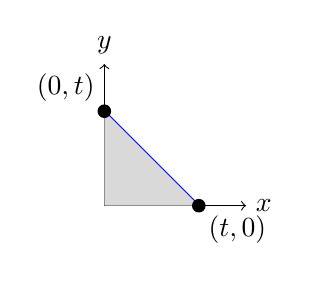
\begin{tikzpicture}[scale=1.5] % 可以调整缩放比例以适应文档
            \def\t{0.8}
            \draw[->] (0,0) -- (1.2,0) node[right] {$x$};
            \draw[->] (0,0) -- (0,1.2) node[above] {$y$};
            \draw[blue, thick] (0,\t) -- (\t,0);
            \fill[gray!30] (0,0) -- (0,\t) -- (\t,0) -- cycle;
            \filldraw (0,\t) circle (1.5pt) node[above left] {$(0, t)$};
            \filldraw (\t,0) circle (1.5pt) node[below right] {$(t, 0)$};
            \end{tikzpicture}
        \end{center}
        \begin{align*}
            \iint_{D_t}f(t)\d x\d y &= \frac{1}{2}t^2f(t) \\
            \iint_{D_t}f'(x+y)\d x\d y 
            &= \int_{0}^{t}\d x\int_{0}^{t-x}f'(x+y)\d y \\
            &= \int_{0}^{t}f(x+y)\bigg|^{y=t-x}_{y=0}\d x \\
            &= \int_{0}^{t}\left[f(t)-f(x)\right]\d x \\
            &=tf(t)-\int_{0}^{t}f(x)\d x
        \end{align*}
        由题即转换为求解如下初值问题
        $$
        \begin{cases}
            tf(t)-\int_{0}^{t}f(x)\d x = \frac{1}{2}t^2f(t) \\
            f(0)= 1 
        \end{cases}
        $$
        可以解出$\displaystyle f(x)=\frac{4}{(x-2)^2}$
    \end{solution}
\end{enumerate}

\ifx\allfiles\undefined
\end{document}
\fi